\section{The geometric Hall algebra}
\label{HallAlgebra}
In this section we outline the construction of the simplicial system of groupoids associated to a category $\CCC$. This system is a variation of the Waldhausen construction studied in \cite{KapranovDyckerhoff} and \cite{Dyckerhoff}, where the authors note that it contains  associativity data of a usual Ringel-Hall algebra and can also be used to construct higher-categorical objects of a similar nature. These constructions are summarily called \emph{transfer theories}. In this paper we are interested in the construction whose end-result is monoidal linear category with braiding obtained by considering linear representations of groupoids. 

We will further recall a variation of Waldhausen construction which we call a geometric Hall algebra from \cite{GeometricHallAlgebra1}. A further extension of the latter in \autoref{Extension} serves as a basis for the construction of the braiding in \autoref{Braiding}. 
%%%%%%%%%%%%%%%%%%%%%%%%%%%%%%%%%%%%%%%%%%%%%%%%%%
\subsection{The Waldhausen S-construction}
\label{Waldhausen}
In this section we recall the variant of the Waldhausen $S$-construction. It was originally introduced by Waldhausen to define the Algebraic K-theory of what are now known as Waldhausen categories. We consider the variant due to Kapranov--Dyckerhoff \cite{KapranovDyckerhoff} that produces a simplicial groupoid associated to an abelian category $\CCC$. 

Note that the classes of mono- and epimorphisms in $\CCC$ satisfy the following: 
 \begin{enumerate}
 \item Any commutative square with monomorphisms as vertical and epimorphisms as horizontal maps is a pullback iff it is a pushout. We will call such squares bicartesian.
  \item Pullbacks and pushouts of monomorphisms along epimorphisms exist.
 \end{enumerate}

In other words the classes of epi- and monomorphisms provide $\CCC$ with a structure of \emph{proto-abelian} category (see \cite{Dyckerhoff} for more details).

Let $X\in\OrdSet$. We consider the marked category $\grid(X):=\Hom_{\Delta}(0\to 1,X)$ with marked objects being the constant maps. Note that $\grid(X)$ has two classes of maps, the "horizontal" and the "vertical", i.e. the maps that are identity respectively on the 0 or 1 component. 

Define $S_X\CCC$ to be the groupoid of maps from $\grid(X)$ to $\CCC$ which take the marked objects to $0$, the horizontal maps to monomorphisms and the vertical maps to epimorphisms, and take Cartesian squares to Cartesian squares.

\begin{Example}
Take $X=\ord{1}=0\to 1$, then \[
\grid(X)=\stik{1}{
00 \ar{r} \& 01 \ar{d} \\
{} \& 11
}
\]
and so $S_X\CCC=S_{\ord{1}}\CCC$ is the groupoid of objects of $\CCC$. 
\end{Example}

\begin{Example}
Take $X=\ord{2}=0\to 1\to 2$, then  \[
\grid(X)=\stik{1}{
00 \ar{r} \& 01 \ar{r} \ar{d} \& 02 \ar{d} \\
{} \& 11 \ar{r} \& 12 \ar{d} \\
{} \& {} \& 22
}
\]
The data of a map $\grid(X)\to\CCC$ then consists of a square\[
\stik{1}{
C_{01} \ar[hook]{r} \ar[two heads]{d} \& C_{02} \ar[two heads]{d}\\
C_{11}=0 \ar[hook]{r} \& C_{12}
}
\]
which must be Cartesian and therefore also coCartesian. This just means that $C_{01}\to C_{02} \to C_{12}$ is an exact sequence.
In all, $S_X\CCC=S_{\ord{2}}\CCC$ is the groupoid of exact sequences in $\CCC$.
\end{Example}
For a general $X=\ord{n}$ we get the groupoid of diagrams of the form 
\[
\stik{1}{
0 \ar[hook]{r} \& C_{01} \ar[two heads]{d} \ar[hook]{r} \& C_{02}\ar[two heads]{d} \ar[hook]{r} \& \cdots  \ar[hook]{r} \& C_{0n}\ar[two heads]{d} \\
{} \& 0  \ar[hook]{r} \& C_{12}\ar[two heads]{d} \ar[hook]{r} \& \cdots  \ar[hook]{r} \& C_{1n}\ar[two heads]{d} \\
{} \& {} \& 0 \ar[hook]{r} \& \cdots  \ar[hook]{r} \& C_{2n}\ar[two heads]{d}\\
{} \& {} \& {} \& \ddots \& \vdots\ar[two heads]{d} \\
{} \& {} \& {} \& {} \& 0
}
\]
where every square is biCartesian.

As shown in \cite{KapranovDyckerhoff} Lemma 2.4.9 the groupoid of diagrams of this shape is equivalent to the groupoid of flags of length $n$.

\lena{we drop the whole mention of needing to consider subcategories for "proto-abelianess" here for the sake of brevity/not mentioning issues we are not fully resolving in the article}

The above formulation of the Waldhausen construction can be extended in an obvious way to provide a functor from the category of simplicial sets $\sset$ to $\Spaces$. For our construction of the candidate for the braiding isomorphism we will need a further extension of this construction to the category of finite distributive lattices $\DLat$ and the presheaves on this category which we call $\lSet$ as discussed in \autoref{ExtWaldhausen}. 

%\begin{Remark}
%This is for Hall algebra section
%It is shown in \cite{KapranovDyckerhoff} that the Waldhausen construction described above is a $2$-Segal space.
%\end{Remark}

\begin{Notation}
In the following sections we will shorten the notation from $S_{[n]}$ to $S_{n}$.
\end{Notation}


%%%%%%%%%%%%%%%%%%%%%%%%%%%%%%%%%%%%%%%%%%%%%%%%%%
\subsection{Recovering the Ringel-Hall algebra}
The spaces $S_1$ and $S_2$ of the Waldhausen construction can be used to define multiplication in the Ringel-Hall algebra associated to the category $\CCC$. Recall that $S_1$ is the groupoid of objects of $\CCC$ and $S_2$ is the groupoid of short exact sequences. We have the maps $mid:S_2 \to S_1$ and $end:S_2 \to S_1\times S_1$ given by 
\begin{align*}
    mid(0\to U\to V\to W\to 0)&=V\\
    end(0\to U\to V\to W\to 0)&=(U,W)
\end{align*}

This defines a correspondence 
\[
\stik{1}{
{} \& S_2 \ar{dl}[above, xshift=-0.5em]{end} \ar{dr}{mid} \& {} \\
S_1\times S_1 \& {} \& S_1
}
\]

This correspondence defines multiplication on the vector space of functions on the set of isomorphism classes of $\CCC$, which recovers the usual construction of the Hall algebra. More precisely, let $\Func(S_1)$ be the $\QQ$-vector space of finitely supported functions on the set of isomorphism classes of the groupoid $S_1$. We can define linear maps of vector spaces $mid_!$ and $end^*$:
\[
mid_!\phi(b)=\sum_{a \in A_b}\frac{\phi(a)}{\Aut(a)}
\]
\[
end^*\phi(a)=\phi(F(a))
\]
where $A_b$ denotes the 2-fiber over $b$. (These are well defined for any finitary abelian $\CCC$ - see \cite{Dyckerhoff} for details). The multiplication on the Ringel-Hall algebra $\Func(S_1)$ is then defined by applying the push-pull construction.

This multiplication can be shown to be associative by considering the associativity square in the category of correspondences. In \cite{Dyckerhoff} it is shown that this square commutes using relations between $S_1,S_2,S_3$ which are an instance of the 2-Segal conditions introduced in \cite{KapranovDyckerhoff}. In fact as discussed there all spaces $S_n$ satisfy these conditions. The upshot is that the higher 2-Segal conditions imply higher associativity conditions when working with constructions leading to a higher categorical versions of Hall algebra. Examples include taking representations of groupoids (instead of functions on them above) in \cite{KapranovDyckerhoff} and sheaves on stacks in \cite{GeometricHallAlgebra1}.

Note that reading the correspodence backwards will give us a comultiplication.

%%%%%%%%%%%%%%%%%%%%%%%%%%%%%%%%%%%%%%%%%%%%%%%%%%%%

\subsection{The geometric Hall algebra}
\label{GeneralHall}
In this section we recap the construction carried out in \cite{GeometricHallAlgebra1}. This can be thought of as the extension of the Waldhausen construction from \autoref{Waldhausen}.

We observe that the underlying structure of two morphisms becomes more transparent if one works in the \lena{double?} category of correspondences $\Corr(\Spaces)$. Working in this category allows one to represent the two-morphisms by certain functorially constructed groupoids. To construct these we extend the Waldhausen construction to the category of simplicial sets. We obtain a functor $H_{geom}:\AugOrdSet \rightarrow \Corr(\Spaces)$. This object is called \emph{the geometric Hall algebra}.

We provide a \emph{transfer theory} for $\Corr(\Spaces)$ in \autoref{Transfer} which in particular recovers the monoidal category$\bigoplus \Rep(\GL(n,\FF_q))$ in $\LinCat$ and \lena{other examples we will consider?}. 

To recover the braiding we extend $H_{geom}$ so it gives an inherently $E_2$-type system in \autoref{Extension}.
%%%%%%%%%%%%%%%%%%%%%%%%%%%%%%%%%%%%%%%%%%%%%%%%%
\subsubsection{The category of correspondences}
\label{Corr}

For $\DDD$ a category we define $\Corr(\DDD)$ to be the double category with both vertical and horizontal morphisms being correspondences (spans) in $\DDD$
\[
\stik{1}{
A \& E \ar{l}{s} \ar{r}{p} \& B
}
\]

2-morphisms are diagrams of the form
\[
\stik{1}{
A \& E \ar{l}{s} \ar{r}{p} \& B \\
F \ar{u}{s} \ar{d}{p}\& Z \ar{u}{s} \ar{d}{p}\ar{l}{s} \ar{r}{p} \& G\ar{u}{s} \ar{d}{p} \\
C \& H \ar{l}{s} \ar{r}{p} \& D \\
}
\]

%%%%%%%%%%%%%%%%%%%%%%%%%%%%%%%%%%%%%%%%%%%%%%%
%%%%%%%%%%%%%%%%%%%%%%%%%%%%%%%%%%%%%%%%%%%%%%%

\subsubsection{The functor $H_{geom}$}
\label{Hallgeom}
Our construction of $H_{geom}:\AugOrdSet \rightarrow \Corr(\Spaces)$ factors through the double category of correspondences in $\sset^{op}$. Let us denote the two parts as \[H_{comb}:\OrdSet\to \Corr(\sset^{op})\] - the combinatorial Hall algebra and \[S^{ext}:\Corr(\sset^{op}) \to \Corr(\Spaces)\] - the extended Waldhausen construction. 

We start from the construction of $H_{comb}$.
\begin{Definition}
For $X\in\AugOrdSet$ define the \emph{augmentation} of $X$, $\aug{X}$ to be $\Hom_\OrdSet(X,0\rightarrow 1)$ considered as an object in $\OrdSet^{op}$.
\end{Definition}

This sends the totally ordered set with $n$ elements in $\AugOrdSet$ (which we denote $\ord{n}$) to the totally ordered set with $n+1$ elements in $\OrdSet^{op}$ (which we also denote $\ord{n}$).

\subsubsection{\texorpdfstring{$H_{comb}$}{Hcomb} on objects}
\label{HcombObjects}
Let $X\in\AugOrdSet$. Each element $x\in X$ determines an embedding of $\aug{\{x\}}$ in $\aug{X}$ as follows: Given a map $\{x\} \to \{0\rightarrow 1\}$, we extend it to a map $X \to \{0 \rightarrow 1\}$ by setting it to $0$ on lower than $x$ elements and $1$ on higher than $x$ elements of $X$. Let $H_{comb}(X)$ be the sub-simplicial set of $\aug{X}$ (considered as an object in $\sset^{op}$) generated by these embeddings.

\begin{Example}
The first few values of $H_{comb}$ on the objects of $\AugOrdSet$ are as follows
\begin{itemize}
\item $H_{comb}(\ord{0})=\ord{0}$
\item $H_{comb}(\ord{1})=\ord{1}$ 
\item $H_{comb}(\ord{2})$ is the horn 
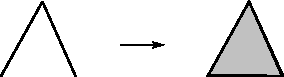
\includegraphics[scale=0.3]{Figures/2HornComb.pdf}
\item $H_{comb}(\ord{3})$ is 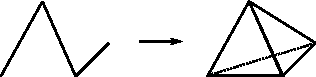
\includegraphics[scale=0.3]{Figures/3HornComb.pdf}
\end{itemize}
\end{Example}

From the description in \autoref{Waldhausen} it is clear how $S$ extends to these objects. Altogether after applying $S$ and the transfer \autoref{VectTransfer} to $\Vect$ $\ord{1}$ goes to the space of functions on the isomorphism classes of objects of $\CCC$, and $\ord{n}$ goes to its $n^{th}$ tensor power presented as functions on isomorphism classes of $n$-tuples of objects.

\subsubsection{\texorpdfstring{$H_{comb}$}{Hcomb} on arrows}

Let $X \xrightarrow{f} Y$ be a map in $\OrdSet$. We want to associate to it a correspondence in $\sset^{op}$.

Let $y\in Y$ and denote $X_y$ the preimage of $y$ under $f$. Similarly to the above, we get an imbedding $\aug{X_y}$ in $\aug{X}$. Denote the sub-simplicial set generated by these imbeddings for all $y$ by $H_{comb}(f)$. Then we have a natural correspondence \[
H_{comb}(X) \rightarrow{} H_{comb}(f) \leftarrow H_{comb}(Y)
\]

\begin{Example}
The multiplication is the image of the map $\ord{2} \to \ord{1}$, and on the level of $H_{comb}$ this map goes to 
\[
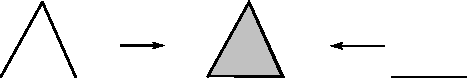
\includegraphics[scale=0.5]{Figures/2MultComb.pdf}
\]
$S^{ext}$ then sends the middle object to the short exact sequences, and the maps to restriction to the endpoints or middle respectively. In all after applying transfer we get the usual multiplication in the Hall algebra.
\end{Example}

%%%%%%%%%%%%%%%%%%%%%%%%%%%%%%%%%%%%%

\subsubsection{\texorpdfstring{$H_{comb}$}{Hcomb} on squares}

Given a square in $\OrdSet$
\[
\stik{1}{
X \ar{r}{f} \ar{d}{g} \& Y \ar{d}{h}\\
Z \ar{r}{k} \& W
}
\]
Similarly to what we did with arrows, we have a map $X\xrightarrow{\alpha}W$ and we then construct the square of correspondences

\[
\stik{1}{
H_{comb}(X) \ar{r} \ar{d} \& H_{comb}(f) \ar{d}{}\& H_{comb}(Y) \ar{l} \ar{d} \\
H_{comb}(g) \ar{r} \& H_{comb}(\alpha) \& H_{comb}(h) \ar{l}{} \\
H_{comb}(Z) \ar{u} \ar{r} \& H_{comb}(k) \ar{u} \& H_{comb}(W) \ar{l} \ar{u}
}
\]

\begin{Example}
\label{AssocInSset}
The associator is the image of the square in $\OrdSet$ \[
\stik{1}{
\ord{3} \ar{r} \ar{d} \& \ord{2} \ar{d} \\
\ord{2} \ar{r} \& \ord{1}
}
\]

Its image under $H_{comb}$ is
\[
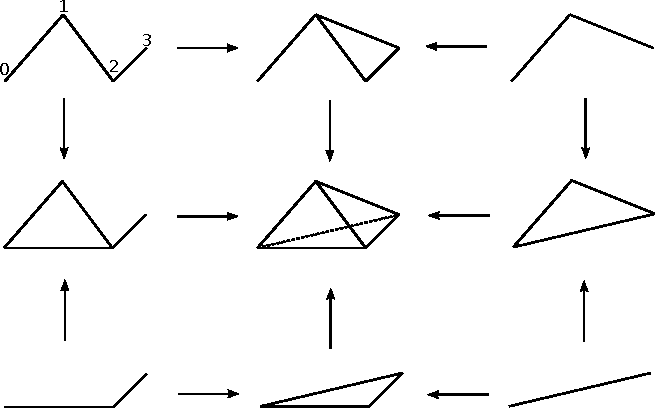
\includegraphics[scale=0.8]{Figures/AssocInSset.pdf}
\]

Note that in order to get associative multiplication after applying transfer construction from \autoref{transfer}, the extended $S$ construction should take the upper right and lower left squares to homotopy pullback squares. This is precisely equivalent to the 2-Segal conditions on $S_3,S_2,S_1$ from \cite{KapranovDyckerhoff}. i.e. that the induced maps
\begin{align*}
    S_{\{0123\}} &\to S_{\{013\}}\times_{S_{\{13\}}}S_{\{123\}}\\
    S_{\{0123\}} &\to S_{\{023\}}\times_{S_{\{02\}}}S_{\{012\}}
\end{align*}
are weak equivalences.
\end{Example}


%%%%%%%%%%%%%%%%%%%%%%%%%%%%%%%%%%%%
